%%%%%%%%%%%%%%%%%%%%%%%%%%%%%%%%%%%%%%%%%%%%%%%%%%%%%%%%%%%%%%%%%%%%%%%%%%%%%%%%%
%Beamer-Präsentationsvorlage
%%%%%%%%%%%%%%%%%%%%%%%%%%%%%%%%%%%%%%%%%%%%%%%%%%%%%%%%%%%%%%%%%%%%%%%%%%%%%%%%%

\documentclass[xcolor=dvipsnames]{beamer}


%\usepackage{xcolor}
\usetheme{default}
\usepackage{qrcode}
% deutsche Silbentrennung
\usepackage[ngerman]{babel}
% Deutsche Umlaute
\usepackage[utf8]{inputenc}
% Einbinden von Bildern
\usepackage{graphicx}
% Unterstützung von Hyperlinks
\usepackage{hyperref}

% Mathematische Pakete
\usepackage{amsmath}
\usepackage{amssymb}
\usepackage{amsfonts}
\usepackage{amsthm}
\usepackage{latexsym}
\usepackage{colortbl}
\usepackage{listings}
\usepackage{booktabs}
% Abweichung von Vorlage
% um Graphen zu plotten
\usepackage{tikz}
\usetikzlibrary{shapes, arrows, automata, chains, positioning, shadows, matrix}



\usepackage{tikzscale}
\usepackage{tikz-uml}\usepackage{tabularx}


\makeatletter
\newcommand{\trickbeamer}{%
	\advance\beamer@slideinframe by-1%
}%
\makeatother



\def \variableXYZ{Ueberschrift1}
\def \variableXYZ{Ueberschrift1}
\newcommand{\neueFolie}[1]{\frametitle{#1}\section{#1}}


\definecolor{rgray}{rgb}{0.95,0.95,0.95}
\definecolor{darkgreen}{rgb}{0.0,0.5,0.0}
\lstset{
	language=[LaTeX]TeX, 
	captionpos=b, 
	frame=lines, 
	basicstyle=\ttfamily, 
	keywordstyle=\color{blue}, 
	commentstyle=\color{darkgreen}, 
	stringstyle=\color{red}, 
	%numbers=left, 
	%numberstyle=\tiny, 
	%numbersep=5pt,
	breaklines=true, 
	showstringspaces=false, 
	emph={double,bool,int,unsigned,char,true,false,void},
	emphstyle=\color{blue},
	emph={Assert,Test},
	emphstyle=\color{red},
	emph={[2]\using,\#define,\#ifdef,\#endif}, 
	emphstyle={[2]\color{blue}},
	backgroundcolor=\color{rgray}
}

\setbeamercolor{frametitle}{fg=black}
\setbeamertemplate{navigation symbols}{}%remove navigation symbols
\setbeamercolor{itemize item}{bg=gray, fg=gray} 
\setbeamercolor{itemize subitem}{fg=gray}
\setbeamercolor{section in toc}{fg=darkgray}
\setbeamercolor{subsection in toc shaded}{fg=gray}
\setbeamercolor{title}{fg=black}
\usepackage{animate}
%\setbeamertemplate{frametitle}
%{
%\includegraphics[width=3cm]{Gestaltung/oth_logo.png}\hfill
%%\parbox{0.6\textwidth}{\color{black}
%%\vspace*{-1cm}{
%\insertframetitle
%%}
%%}
%\hspace*{-0.3cm}\color{black}\rule{20cm}{0.2mm}
%}

\setbeamertemplate{frametitle}
{% 
%\vspace{-0.165ex} 
\begin{beamercolorbox}[wd=\paperwidth,dp=1ex, ht=4ex, sep=0.5ex, colsep*=0pt]{frametitle}% 
    \usebeamerfont{frametitle}   \strut 
    \raisebox{-0.55ex}[0pt][-\ht\strutbox ]{
    	
\includegraphics[width=1.7cm]{Gestaltung/Logo_Hochschule_Ansbach.png}
    	}  
    \hfill  \insertframetitle \hspace{0.4cm}
    \end{beamercolorbox}
    \vspace*{-0.5cm}
    \hspace*{-2cm}
\color{black}\rule{15cm}{0.2mm}               
}%


%\setbeamertemplate{headline}{
%\begin{beamercolorbox}{frametitle}


%\begin{flushright}

%\end{flushright}
%}} 
%\end{beamercolorbox}%

%}
\setbeamertemplate{footline}
{
  \leavevmode%
  \vspace*{0.2cm}
     \hspace*{-2cm}
	\color{black}\rule{15cm}{0.2mm}   
  \hbox{%
  \begin{beamercolorbox}[wd=1.15\paperwidth,ht=1.5ex,dp=1ex, center]{author in head/foot}%
    \usebeamerfont{author in head/foot}\color{black}\insertshortauthor \hfill
\insertshorttitle  \hfill    Seite \insertframenumber /\inserttotalframenumber
\vspace*{0.02cm}
  \end{beamercolorbox}}%
}

\setbeamerfont{tiny structure}{size=\tiny}


\defbeamertemplate*{title page}{customized}[1][]
{
\begin{minipage}{0.8\linewidth}
  \usebeamerfont{title}\inserttitle\par
  \usebeamerfont{subtitle}\usebeamercolor[fg]{subtitle}\insertsubtitle\par
  \bigskip
  \usebeamerfont{author}\insertauthor\par
  \usebeamerfont{institute}\insertinstitute\par
  \usebeamerfont{date}\insertdate\par
  %\usebeamercolor[fg]{titlegraphic}\inserttitlegraphic
\end{minipage} \hfill
\begin{minipage}{0.15\linewidth}
  \vspace*{0pt}
  \usebeamercolor[fg]{titlegraphic}\inserttitlegraphic
\end{minipage}
  
  
}

%%%%%%%%%%%%%%%%%%%%%%%%%%%%%%%%%%%%%%%%%%%%%%%%%%%%%%%%%%%%%%%%%%%%%%%%%%%%%%%%%
%Hier werden die Daten für die erste Folie eingetragen
%%%%%%%%%%%%%%%%%%%%%%%%%%%%%%%%%%%%%%%%%%%%%%%%%%%%%%%%%%%%%%%%%%%%%%%%%%%%%%%%%
\title{Werkzeuge für das Erstellen von UML-Diagrammen}
\subtitle{Open-Source Software for the Working Scientist \\}
\institute{Master of Applied Research\\ Hochschule Ansbach\\}
\author{Marco Obermeier}
\date{\today}
%\date{12. Januar 2022}

\begin{document} 
	\begin{frame}
		\frametitle{~}
		\maketitle 
	\end{frame}
	%%%%%%%%%%%%%%%%%%%%%%%%%%%%%%%%%%%%%%%%%%%%%%%%%%%%%%%%%%%%%%%%%%%%%%%%%%%%%%%%%
	%Einleitung
	%%%%%%%%%%%%%%%%%%%%%%%%%%%%%%%%%%%%%%%%%%%%%%%%%%%%%%%%%%%%%%%%%%%%%%%%%%%%%%%%%
	\begin{frame}
		\frametitle{Inhaltsverzeichnis}
		\tableofcontents
	\end{frame}
	
	
	%%%%%%%%%%%%%%%%%%%%%%%%%%%%%%%%%%%%%%%%%%%%%%%%%%%%%%%%%%%%%%%%%%%%%%%%%%%%%%%%%
	%Introduction
	%%%%%%%%%%%%%%%%%%%%%%%%%%%%%%%%%%%%%%%%%%%%%%%%%%%%%%%%%%%%%%%%%%%%%%%%%%%%%%%%%
	\small
	\begin{frame}
		\section{Einführung}
		\frametitle{Einführung}
		\begin{columns}
			\begin{column}{0.50\textwidth}
				\begin{block}{Campus Feuchtwangen}
					\begin{itemize}
						\item Entwicklung eines Smart Energy Systems
						\item Intelligente Nutzung nachhaltiger Gebäudetechnik
						\item Intelligenter Bezug vom Stromnetz und Einspeisung
						\item Großer Softwareanteil
					\end{itemize}
				\end{block}
			\end{column}
			
			\begin{column}{0.50\textwidth}
				\begin{block}{Professionelle Entwicklung}
					\begin{itemize}
						\item Struktierte Software
						\item Softwareentwicklung im Team und nachvollziehbare Dokumentation
						\item Einsatz von UML-Diagrammen (unified modeling language)
					\end{itemize}
				\end{block}
			\end{column}
		\end{columns}
		
	\end{frame}
	
	
	
	
	
	%%%%%%%%%%%%%%%%%%%%%%%%%%%%%%%%%%%%%%%%%%%%%%%%%%%%%%%%%%%%%%%%%%%%%%%%%%%%%%%%%
	%UML Diagramme
	%%%%%%%%%%%%%%%%%%%%%%%%%%%%%%%%%%%%%%%%%%%%%%%%%%%%%%%%%%%%%%%%%%%%%%%%%%%%%%%%%
	\begin{frame}
		\section{Theoretischer Hintergrund}
		\frametitle{Theoretischer Hintergrund: UML-Diagramme}
		\begin{columns}
			\begin{column}{0.50\textwidth}
				\begin{block}{Was ist UML?}
					\begin{itemize}
						\item Standard im Software Engineering
						\item Zusammenstellung verschiedener Modellierungstechniken und Diagrammen
					\end{itemize}
				\end{block}
			\end{column}
			
			\begin{column}{0.50\textwidth}
				\begin{block}{Beispiel Komponentendiagramm}
						\begin{itemize}
							\item Logische Komponenten und physische Komponenten 
							\item Schnittstellen und Zusammenhang zwischen Komponenten
						\end{itemize}
					\begin{minipage}{1.0\textwidth}	
						\resizebox{\columnwidth}{!}{
					\begin{tikzpicture}
						
						% Komponenten
						\umlbasiccomponent[x=0,y=0]{Komponente 1}
						\umlbasiccomponent[x=6,y=0]{Komponente 2}

						% Verbindungen
						\umlassemblyconnector[interface= Schnittstelle 1]{Komponente 1}{Komponente 2}
						
					\end{tikzpicture}
				}
			\end{minipage}
		
				\end{block}
			\end{column}
		\end{columns}
		\begin{thebibliography}{00}
			\tiny
			\bibliographystyle{IEEEtran}
			\bibitem{b1}Akkøk, M. An overview of the unified modeling language and diagrammatic modeling language design in software engineering. {\em Information Design Journal}. \textbf{11}, 151-159 (2002), \url{https://www.jbe-platform.com/content/journals/10.1075/idj.11.2.07akk}
			\bibitem{b2} Fakhroutdinov, Kirill. “UML 2.5 Diagrams Overview.” UML Diagrams - Overview, Reference, and Examples., 25 Nov. 2013, \url{https://www.uml-diagrams.org/uml-25-diagrams.html} 
			
		\end{thebibliography}
	\end{frame}
	
	
	
	
	
	%%%%%%%%%%%%%%%%%%%%%%%%%%%%%%%%%%%%%%%%%%%%%%%%%%%%%%%%%%%%%%%%%%%%%%%%%%%%%%%%%
	%UML Diagramme
	%%%%%%%%%%%%%%%%%%%%%%%%%%%%%%%%%%%%%%%%%%%%%%%%%%%%%%%%%%%%%%%%%%%%%%%%%%%%%%%%%
	\begin{frame}
		\frametitle{Untersuchtes Diagramm des Forschungsprojekts}
		\begin{columns}
			
			
			\begin{column}{0.35\textwidth}
				\begin{block}{Untersuchtes Diagramm}
					\begin{itemize}
						\item Komponentendiagramm des Energiemanagementsystem
						\item Blaue Komponenten sind im Fokus der Forschung
						\item Gelbe Komponenten sind bereits implementiert
					\end{itemize}
					
				\end{block}
			\end{column}
	
			\begin{column}{0.7\textwidth}
				\begin{minipage}{\textwidth}
					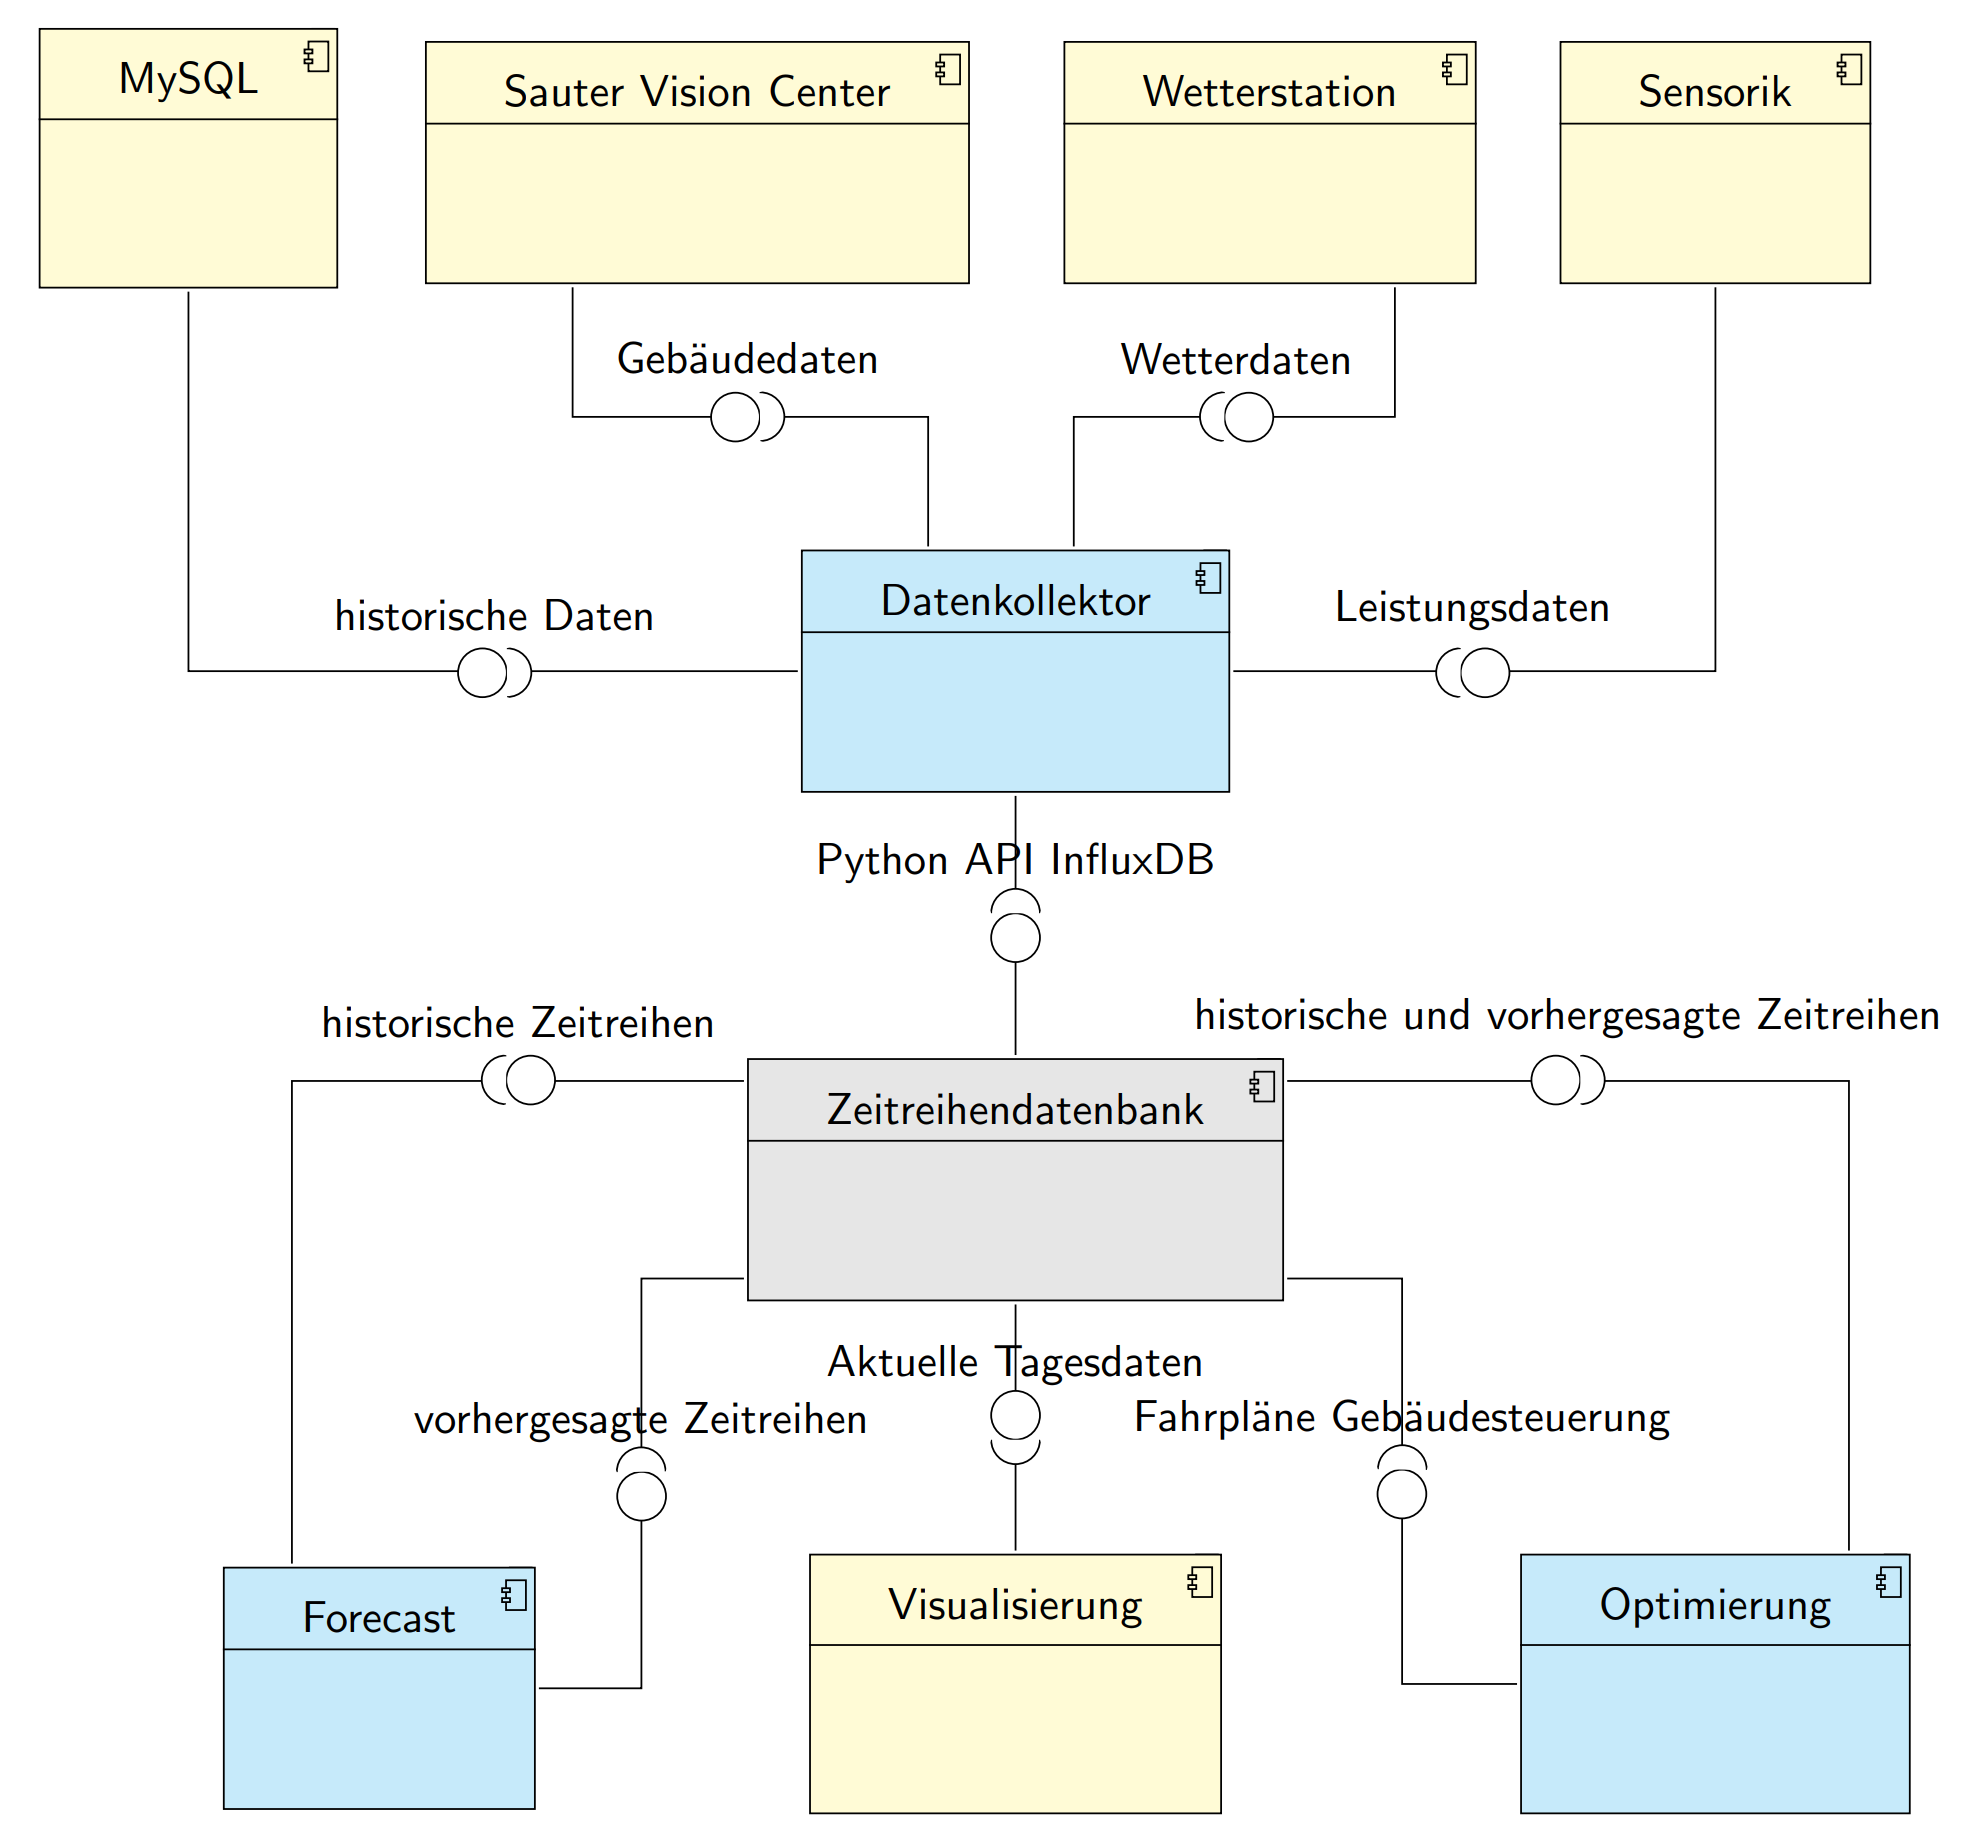
\includegraphics[scale=0.25]{../Diagramms/Hand/uml.PNG}
				\end{minipage}
			\end{column}
			
				\end{columns}
	\end{frame}
	
	
	
	%%%%%%%%%%%%%%%%%%%%%%%%%%%%%%%%%%%%%%%%%%%%%%%%%%%%%%%%%%%%%%%%%%%%%%%%%%%%%%%%%
%UML Diagramme
%%%%%%%%%%%%%%%%%%%%%%%%%%%%%%%%%%%%%%%%%%%%%%%%%%%%%%%%%%%%%%%%%%%%%%%%%%%%%%%%%
\begin{frame}
	\frametitle{Use Cases \& Untersuchungskriterien}
	\begin{block}{Use Cases der Werkezeuge für UML-Diagramme}
		\begin{itemize}
			\item Zusammenarbeit mit anderen Wissenschaftlern überwiegend für Konzepte - klare Abgrenzung von detailierten Diagrammen
			\item Klare und saubere Darstellung in Veröffentlichungen
		\end{itemize}
		
	\end{block}
	\begin{table}
		\begin{tabular}{l l}
			\toprule
			\textbf{Untersuchungskriterium} & \textbf{Beschreibung der Bewertung}\\
			\midrule
			Zeitaufwand für die Erstellung & Zeit in Stunden \\
			\midrule
			Zeitaufwand für das Abändern & Zeit in Minuten für das hinzufügen  \\
			& einer Komponente \\
			\midrule
			Allgemeiner visueller Eindruck & Bewertung nach Schulnoten\\
			\midrule
			Plattformunabhängigkeit &
			Lauffähig auf Windows, Linux, MacOS ? \\
			\midrule
			Skalierbarkeit der Diagrammgröße & Ist die Übersichtlichkeit bei steigender  \\
			& Diagrammgröße leicht handlebar? \\
			\bottomrule
		\end{tabular}
	\end{table}
	
	
	
\end{frame}




%%%%%%%%%%%%%%%%%%%%%%%%%%%%%%%%%%%%%%%%%%%%%%%%%%%%%%%%%%%%%%%%%%%%%%%%%%%%%%%%%
%UML Diagramme
%%%%%%%%%%%%%%%%%%%%%%%%%%%%%%%%%%%%%%%%%%%%%%%%%%%%%%%%%%%%%%%%%%%%%%%%%%%%%%%%%
\begin{frame}
	\frametitle{Auswahl der Softwarewerkzeuge}

\begin{block}{Ausgewählte Softwarewerkzeuge:}
	\begin{itemize}
		\item Grobe Vorauswahl gemäßg den Use-Cases
		\item Berücksichtigung der Platformunabhänigkeit
	\end{itemize}
\end{block}


\begin{columns}
	\begin{column}{0.333\textwidth}
		\begin{block}{\textbf{Tikz-UML}}
			\begin{itemize}
				\item Textbasiert
				\item Nicht ausschließlich für UML (Latex Paket)
			\end{itemize}
		\end{block}
	\end{column}
	
	\begin{column}{0.333\textwidth}
		\begin{block}{\textbf{Plant UML}}
			\begin{itemize}
				\item Textbasiert
				\item Ausschließlich für UML
			\end{itemize}
		\end{block}
	\end{column}

\begin{column}{0.333\textwidth}
	\begin{block}{\textbf{Draw.IO}}
		\begin{itemize}
			\item Grafische Nutzeroberfläche
			\item Nicht ausschließlich für UML (UML Symbolreiter)
		\end{itemize}
	\end{block}
\end{column}

\end{columns}
	
	
\end{frame}




	%%%%%%%%%%%%%%%%%%%%%%%%%%%%%%%%%%%%%%%%%%%%%%%%%%%%%%%%%%%%%%%%%%%%%%%%%%%%%%%%%
	%Tikz-UML
	%%%%%%%%%%%%%%%%%%%%%%%%%%%%%%%%%%%%%%%%%%%%%%%%%%%%%%%%%%%%%%%%%%%%%%%%%%%%%%%%%
\begin{frame}
	\frametitle{Untersuchungsergebnisse - Tikz-UML}
	\begin{columns}
		\begin{column}{0.30\textwidth}
		\begin{block}{}
			\begin{itemize}
				\item Zeitaufwand für die Erstellung: 4 h
				\item Zeitaufwand für eine Änderung: 10 min
				\item Allgmeiner visueller Eindruck: 2
				\item Skalierbarkeit der Diagrammgröße: nein
				
			\end{itemize}
			
			
		\end{block}
	\end{column}
		
		
		\begin{column}{0.70\textwidth}
			\begin{minipage}{1.0\textwidth}	
				\resizebox{\columnwidth}{!}{%
					\begin{tikzpicture}
						
					
						\umlbasiccomponent[x=0, y=0, fill=yellow!20]{MySQL} 
						\umlbasiccomponent[x=4, y=0,fill=yellow!20]{Sauter Vision Center}
						\umlbasiccomponent[x=8.5, y=0,fill=yellow!20]{Wetterstation}
						\umlbasiccomponent[x=12, y=0,fill=yellow!20]{Sensorik}
						\umlbasiccomponent[x=6.5, y=-4, fill=cyan!20]{Datenkollektor} 
						\umlbasiccomponent[x=6.5, y=-8, fill=gray!20]{Zeitreihendatenbank}
						\umlbasiccomponent[x=1.5, y=-12, fill=cyan!20]{Forecast}
						\umlbasiccomponent[x=6.5, y=-12]{Visualisierung}
						\umlbasiccomponent[x=12, y=-12, fill=cyan!20]{Optimierung}
			
						\umlHVassemblyconnector[interface=historische Daten, anchor1=180,  first arm=1.5cm]{Datenkollektor}{MySQL}
						\umlVHVassemblyconnector[interface={Gebäudedaten}, anchor1=125, anchor2=-135]{Datenkollektor}{Sauter Vision Center}
						\umlVHVassemblyconnector[interface={Wetterdaten}, anchor1=65, anchor2=-45]{Datenkollektor}{Wetterstation}
						\umlHVassemblyconnector[interface=Leistungsdaten, anchor1=0,  first arm=1.5cm]{Datenkollektor}{Sensorik}
						\umlVHVassemblyconnector[interface=Python API InfluxDB, anchor1=90]{Zeitreihendatenbank}{Datenkollektor}
						\umlHVHassemblyconnector[interface=vorhergesagte Zeitreihen, anchor1=-160, anchor2 = 0]{Zeitreihendatenbank}{Forecast}
						\umlVHassemblyconnector[interface=historische Zeitreihen, anchor1=125, anchor2 = -200]{Forecast}{Zeitreihendatenbank}Forecast
						
						\umlVHVassemblyconnector[interface=Aktuelle Tagesdaten, anchor1=-90]{Zeitreihendatenbank}{Visualisierung}
						\umlHVHassemblyconnector[interface=Fahrpläne Gebäudesteuerung, anchor1=-20, anchor2= 180]{Zeitreihendatenbank}{Optimierung}
						\umlVHassemblyconnector[interface={historische und vorhergesagte Zeitreihen}, anchor1=45, anchor2= 20, arm1=3cm]{Optimierung}{Zeitreihendatenbank}
						
						
						
						%\umlVHVassemblyconnector[interface=3D-Beschleunigung, anchor1=0,  first arm=3.5cm]{MySQL}{Datenkollektor}
						%\umlassemblyconnector[interface=Winkelgeschwidigkeit, anchor1=0]{Flugsteuerung}{Gyrosensor}
						%\umlHVHassemblyconnector[interface=PWM-Signal, anchor1=-62,  first arm=3.5cm]{Flugsteuerung}{Motoren}
		
						%\umlVHVassemblyconnector[interface=Lagewinkel]{Regelung}{Sensorauswertung} 
						%\umlVHVassemblyconnector[interface=Motordrehzahl]{Motorsteuerung}{Regelung} 
						
						
					\end{tikzpicture}
				}
			\end{minipage}
		\end{column}
	\end{columns}
\end{frame}



%%%%%%%%%%%%%%%%%%%%%%%%%%%%%%%%%%%%%%%%%%%%%%%%%%%%%%%%%%%%%%%%%%%%%%%%%%%%%%%%%
%Plant UML
%%%%%%%%%%%%%%%%%%%%%%%%%%%%%%%%%%%%%%%%%%%%%%%%%%%%%%%%%%%%%%%%%%%%%%%%%%%%%%%%%
\begin{frame}
	\frametitle{Untersuchungsergebnisse - Plant UML}
	\begin{columns}
		
		\begin{column}{0.35\textwidth}
			\begin{block}{}
				\begin{itemize}
					\item Zeitaufwand für die Erstellung: 2 h
					\item Zeitaufwand für eine Änderung: 5-15 min
					\item Allgmeiner visueller Eindruck: 4
					\item Skalierbarkeit der Diagrammgröße: nein
					
				\end{itemize}
				
			\end{block}
		\end{column}

		
		\begin{column}{0.75\textwidth}
			\begin{minipage}{\textwidth}
				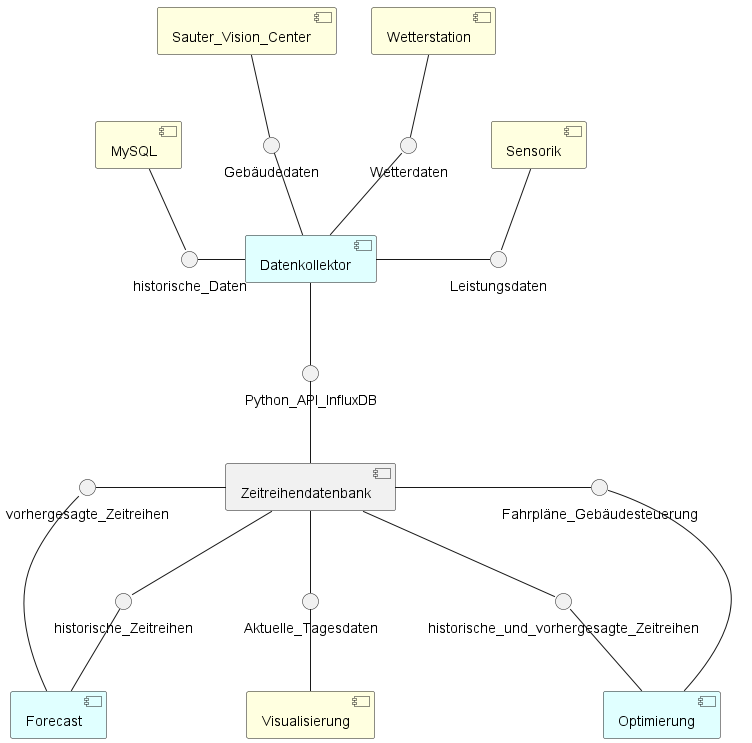
\includegraphics[scale=0.3]{../Diagramms/PlantUML/overview.PNG}
			\end{minipage}
		\end{column}
		
	\end{columns}
\end{frame}



%%%%%%%%%%%%%%%%%%%%%%%%%%%%%%%%%%%%%%%%%%%%%%%%%%%%%%%%%%%%%%%%%%%%%%%%%%%%%%%%%
%Draw.IO
%%%%%%%%%%%%%%%%%%%%%%%%%%%%%%%%%%%%%%%%%%%%%%%%%%%%%%%%%%%%%%%%%%%%%%%%%%%%%%%%%
\begin{frame}
	\frametitle{Untersuchungsergebnisse - Draw.IO}
	\begin{columns}
	
		
		\begin{column}{0.35\textwidth}
			\begin{block}{Untersuchtes Diagramm}
				\begin{block}{}
					\begin{itemize}
						\item Zeitaufwand für die Erstellung: 2,5 h
						\item Zeitaufwand für eine Änderung: 10 min
						\item Allgmeiner visueller Eindruck: 1
						\item Skalierbarkeit der Diagrammgröße: ja
						
					\end{itemize}
					
				\end{block}
				
			\end{block}
		\end{column}
	
		\begin{column}{0.75\textwidth}
		\begin{minipage}{\textwidth}
			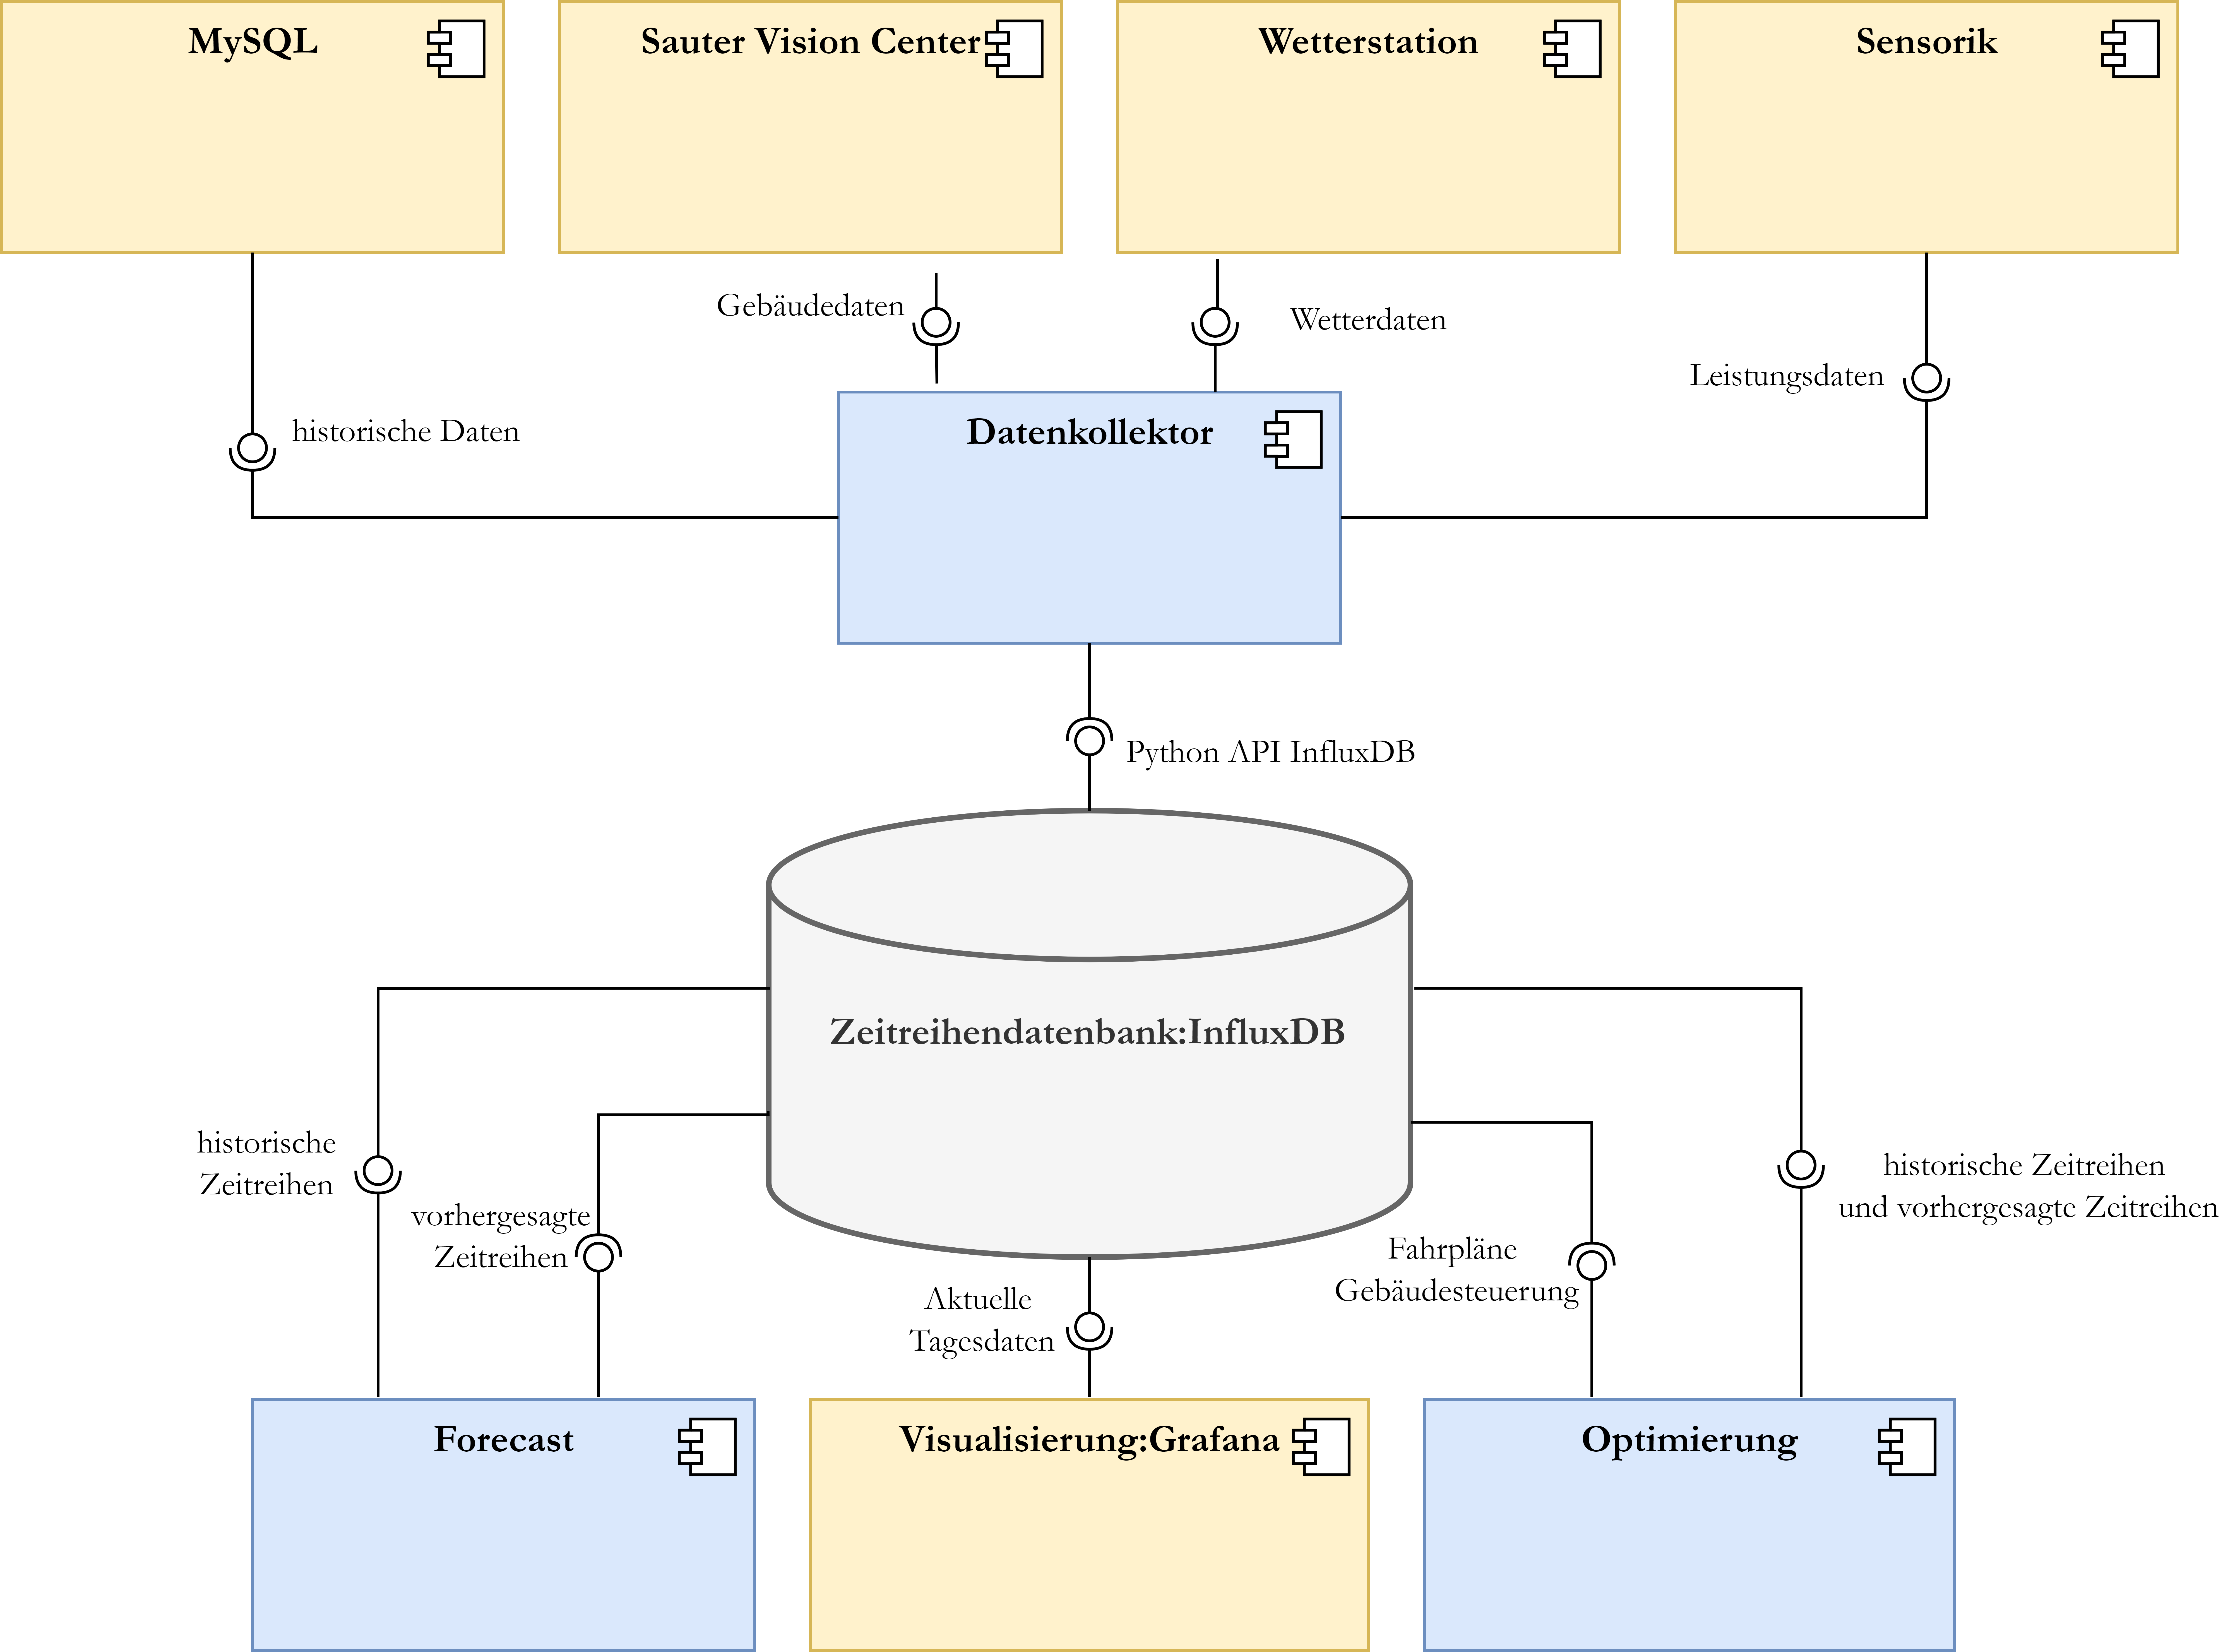
\includegraphics[scale=0.029]{../Diagramms/DrawIO/uml.PNG}
		\end{minipage}
	\end{column}
	\end{columns}
\end{frame}





%%%%%%%%%%%%%%%%%%%%%%%%%%%%%%%%%%%%%%%%%%%%%%%%%%%%%%%%%%%%%%%%%%%%%%%%%%%%%%%%%
%Zusammenfassung 
%%%%%%%%%%%%%%%%%%%%%%%%%%%%%%%%%%%%%%%%%%%%%%%%%%%%%%%%%%%%%%%%%%%%%%%%%%%%%%%%%
\begin{frame}
	\frametitle{Zusammenfassung}
	\begin{columns}
	
			
			\begin{column}{0.33\textwidth}
				\begin{block}{\textbf{Draw.IO}}
					\begin{itemize}
						\item [+] Zusätzliche Symbole
						\item [-] Positionierung Zeitaufwändig
						\item[+] WebApp und VS-Code
					\end{itemize}
				\end{block}
			\end{column}

		\begin{column}{0.4\textwidth}
			\begin{block}{\textbf{Plant UML}}
				\begin{itemize}
					\item[--] Positionierung problematisch
					\item[--] Beschriftung nicht verschiebbar
					\item[+] WebApp und VS-Code
				\end{itemize}
			\end{block}
		\end{column}
		
		\begin{column}{0.33\textwidth}
			\begin{block}{\textbf{Tikz-UML}}
				\begin{itemize}
					\item Positierung nach X, Y - Symmetrie
					\item[+] Integrierbar in Latex-Dokument 
					\item[--] Beschriftung unverschiebbar
				\end{itemize}
			\end{block}
		\end{column}
		
	\end{columns}
	\begin{table}
		\begin{tabular}{l l l l l}
			\toprule
			\textbf{Untersuchungskriterium} & \textbf{Draw.IO} & \textbf{PlantUML} & \textbf{Tikz-UML}\\
			\midrule
			Zeitaufwand für die Erstellung & 2,5 & 2 & 4 \\
			\midrule
			Zeitaufwand für das Abändern & 5 & 5-15 & 10  \\
			\midrule
			Allgemeiner visueller Eindruck & 1 & 4 & 2 \\
			\midrule
			Plattformunabhängigkeit & ja & ja & ja\\
			\midrule
			Skalierbarkeit der Diagrammgröße & ja & nein & nein\\
			\bottomrule
		\end{tabular}
	\end{table}
	
	
	
\end{frame}


%%%%%%%%%%%%%%%%%%%%%%%%%%%%%%%%%%%%%%%%%%%%%%%%%%%%%%%%%%%%%%%%%%%%%%%%%%%%%%%%%
%Empfelungen
%%%%%%%%%%%%%%%%%%%%%%%%%%%%%%%%%%%%%%%%%%%%%%%%%%%%%%%%%%%%%%%%%%%%%%%%%%%%%%%%%
\begin{frame}
	\frametitle{Empfehlungen}
	\begin{columns}
		
		
		\begin{column}{0.33\textwidth}
			\begin{block}{\textbf{Draw.IO}}
				\begin{itemize}
					\item Für Zusammenarbeit in Projekt gut geeignet
				\end{itemize}
			\end{block}
		\end{column}
		
		\begin{column}{0.4\textwidth}
			\begin{block}{\textbf{Plant UML}}
				\begin{itemize}
					\item Für sehr kleine Diagramme in Github
				\end{itemize}
			\end{block}
		\end{column}
		
		\begin{column}{0.33\textwidth}
			\begin{block}{\textbf{Tikz-UML}}
				\begin{itemize}
					\item Für Veröffentlichungen
				\end{itemize}
			\end{block}
		\end{column}
		
	\end{columns}

\end{frame}


%%%%%%%%%%%%%%%%%%%%%%%%%%%%%%%%%%%%%%%%%%%%%%%%%%%%%%%%%%%%%%%%%%%%%%%%%%%%%%%%%
%Introduction
%%%%%%%%%%%%%%%%%%%%%%%%%%%%%%%%%%%%%%%%%%%%%%%%%%%%%%%%%%%%%%%%%%%%%%%%%%%%%%%%%
\begin{frame}
	\frametitle{Ergebnisse und Quellcode Verfügbar auf Github}
	
	\qrcode[height=3in]{https://github.com/OberMarco/OpenSourceSoftwareUML}
	
\end{frame}
	
	
\end{document}